\subsection{Sicherheit}\label{sec:sicherheit}

\subsubsection{Notausschalter}
Ein Notausschalter sogt dafür, dass das Gyroskop im Notfall sofort ausgeschalten werden kann. Um den Notaus zu implementieren gib es 2 verschiedene Möglichkeiten, eine Softwarelösung und eine Hardwarelösung. Beide Möglichkeiten haben ihre Vor- und Nachtteile und diese werden genauer beschrieben.\\
\vspace{3mm}
Bei der Hardwarelösung wird durch Betätigen des Schalters die Spannungsversorgung vom Netzteil unterbrochen und der Motor stoppt. Die Implementation wäre sehr einfach, doch bei der Hardwarelösung  ist das Problem, wenn der Notaus wieder entriegelt wird, der Motor sofort wieder zu drehen beginnt.\\
\vspace{3mm}
Bei der Softwarelösung wird der Notausschalter mit dem Raspberry Pi verbunden und bei Betätigen des Tasters erkennt der Raspberry ein Low Input an einem GPIO-Pin und schaltet der Motor aus. Diese Version ist aber nicht zuverlässig genug, denn wenn der Raspberry eine Störung hat oder das Input Signal nicht erkannt wird, dreht sich das Gyroskop weiter und stellt somit eine Gefahr für den Satelliten dar. Der Vorteil dieser Variante ist, dass programmiert werden kann, dass der Motor nach Entriegelung des Notaus nicht automatisch wieder gestartet wird.\\
\vspace{3mm}
Da beide Lösungen wichtige Funktionen haben, werden die beiden Variante miteinander verbunden. Der Notausschalter wird zwischen die Spannungsversorgung verbunden und mit einem Relais, das an den Raspberry Pi geschlossen wird, wird der Zustand geprüft. Wird der Notausschalter gedrückt, muss mit einem Software Button das Relais wieder geöffnet werden. Durch diese Implementierung wird ein automatisches Starten nach Entriegelung des Notausschalter verhindert. Dies nennt man quittieren, was so viel bedeutet wie bestätigen. Damit man im User Interface um quittieren erinnert wird, blinkt der Quittierungsbutton ROT. 
\pagebreak
\subsubsection{Schlüsselschalter}
Damit nicht jeder die Berechtigung hat, die Teststation in Betrieb zu nehme, wird ein Schlüsselschalter eingebaut. Wird mit dem Schlüssel der Schalter gedreht, hat man den vollen Zugriff auf die Steuerung mit dem Raspberry Pi. \\
\vspace{3mm}
\begin{figure}[H]
    \centering
    \includegraphics[scale=0.8]{image/schlüsselschalter.jpg}
    \caption{Schlüsselschalter}
    \label{fig:enter-label}
\end{figure}
\subsubsection{Endschalter}
Endschalter sind Schalter, die Endposition eines mechanischen Systems erfassen. Sie kommen in verschiedenen Anwendungen wie Maschinenbau, Automatisierungstechnik und Robotik zum Einsatz, um das Erreichen eines bestimmten Punktes zu erkennen. Ihre Verwendung trägt zur Sicherheit und Effizienz von Maschinen und Systemen bei, indem sie das Erreichen der Endpunkte von Bewegungen oder Prozessen signalisieren.\\
\vspace{3mm}
Verkabelung und Befestigung:
Im Rahmen gibt es zwei kleine Aussparungen, in denen die Endschalter platziert werden. Wird nun die Tür geschlossen, werden die Schalter betätigt.\\
\vspace{5mm}
\begin{figure}[H]
    \centering
    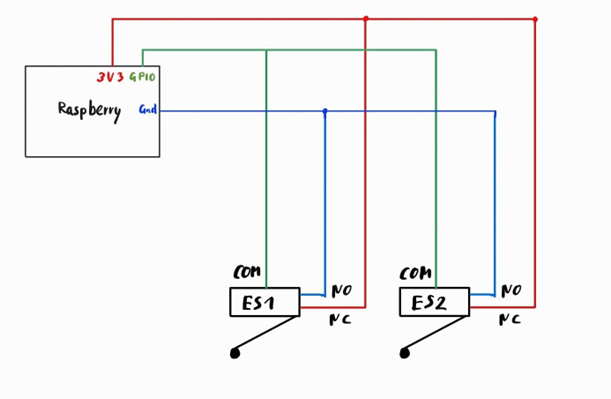
\includegraphics{image/Zusammenschaltung-Endschalter.png}
    \caption{Zusammenschaltung Endschalter}
    \label{fig:enter-label}
\end{figure}
Wenn die Teststation während einem Test bewegt wird, könnten durch die Erschütterungen die Endschalter elektrische Störungen erkennen. Um dies zu verhindern, müssen die Endschalter mindestens eine Sekunde lang das jeweilige Signal erkennen. 

